\chapter{Introduction}
\label{chap:introduction}

Sequencing (reading) a larger genome in one piece still belongs to very expensive, or even hardly possible, tasks. Fortunately, a much cheaper approach exist and is widely used in todays genome sequencing. Its core lies in chopping the genome (or the part of interest) into many short sequences, called reads, and their later assembly into the original sequence. The shorter the reads are, the lower the cost of their reading is. 

Howerver, short reads make the task of their assembly more complicated. Unlike the genome chopping phase, the reads assembly stage would execute purely in software if a mathematical model, properly describing the genome sequencing, existed. Since such models were developed, various genome assembly algorithms were implemented.

We start a description of ideal sequencing data and mathematical model behind the assembly. Next, we explain that the real world is not so bright as the model may indicate. FInal section of this chapter is dedicated to description of two main approaches used by todays assembly algorithms, and to definition of the main goal of this work --- to implement ou own assembly algorithm.

\section{Basic Terms}
\label{sec:basic-terms}

For the rest of this thesis, a genome is viewed as a string of character, each describe a nucleotide, at certain position. Since DNA molecules consist of four types of nucleotides, only four characters, \texttt{A}, \texttt{C}, \texttt{G} or \texttt{T}, appear in the string. Usually, a term base is used as a synonym for nucleotides.

Although we do not know contents of the genome string (since its sequencing is exactly the task for assembly algorithms), we still know its approximate length. Since this thesis focuses on human genome assembly, we expect the genome length around 3 billions of bases (gigabases, Gb). As stated in the beginning of the chapter, the genome to be read is chopped into a large amount of short strings, called reads. In an ideal case, we expect all reads to be of the same length, much lower than the genome string. Usually, read length does not exceed several hundred bases. 

For some species, including humans, a so-called \textit{reference} genome (or sequence) is available. Ideally, it is a fully sequenced (assembled) genome of one individual. SInce genomes of other individuals of the same species show great similarity, the reference may prove being an useful input for an assembly algorithm. 

Some assembly algorithm transform each read into a sequence of \textit{k-mers}, a very short strings of equal length. The read sequence of length $k$ is divided into $l - k + 1$ k-mers $k_0, ..., k_{l-k}$ of length $k$. If we denote bases in the read as $b_0, ..., b_{l-1}$, the k-mer $k_i$ covers bases from $b_i$ to $b_{i+k-1}$. Such definition implies that adjacent k-mers overlap by $k-1$ bases. 

An example of transforming e sequence \texttt{TACTGGCC} into k-mers of length $3$ is ilustrated on Figure \ref{fig:seq-division}. The sequence has $8$ bases in length and $6$ k-mers are created from it. The read sequence, as in all other figures in this work, is marked red, contents of individual k-mers is in yellow.

\begin{figure}[h]
	\centering
	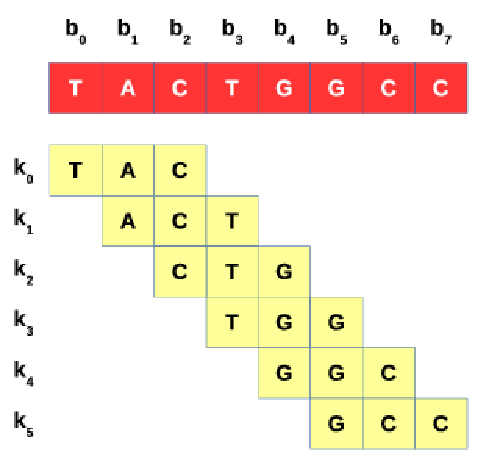
\includegraphics{img/seq-division.pdf}
	\caption{Sequence transformation into k-mers}
	\label{fig:seq-division}
\end{figure}

\section{The Model}
\label{sec:the-model}

The simplest mathematical assembly model, assumes that we are assembling genome string of length $g$, given a set of $n$ reads of length $l$ ($l << g$), each potentialy transformed into a sequence of $l-k+1$ k-mers. The model assumes that bases are, from the genome string, sampled uniformly and randomly and that no errors were produced during the sampling (in other words, all reads contain no misread bases). Since the probability of sampling a base at certain genome position is very low for single sampling event, and the number of sampling events is quite large, the problem of genome base coverage depth (i.e. number of times each base in the genome string appears in reads) follows a Poisson distribution. In other words, the probability that base at certain position is sampled $k$ times is
$$
\frac{c^k}{k!}*e^{-c}
$$
$c$ is a base coverage depth, also known as sequencing depth, and can be computed simply as a total number of bases within the input read set divided by the length of the genome.
$$
c = \frac{n * l}{g}
$$
Very similar relations apply for k-mer coverage depth, only the formula for the k-mer coverage depth needs to be changed to $\frac{n*(l - k + 1)}{g - k + 1}$. These details brings answers to at least two important problems: how many reads need to be created to (statistically) cover the whole genome string, and how to determine whether a given read set is free of sequencing errors?

The percentage of genome not covered by any read from the set is equal to $P(k=0) = e^{-c}$. Multiplying it by the genome size $g$ gives us the number of uncovered bases. So, to cover the whole genome, this number must be lower than $1$ which places condition of $c > ln g$. For example, to cover the whole human genome ($g = 3 * 10^9$), the read coverage depth must be at least $22$. 

Solution to the second problem is implied by the facts that k-mer coverage of the genome follows a Poisson distribution, and that all the theory above was made with an assumption of no sequencing errors. In an ideal case, the k-mer frequency distribution function of an error-free read set would follow the probability mass function of the Poisson distribution, meaning that frequencies of most of the k-mers are near the k-mer coverage depth. However, when we introduce possibility of sequencing errors, it happens that some k-mers would be sampled less often and some become even unique. The k-mer frequency distribution of such a read set does not follow the Poisson distribution. The aspect of sequencing errors and their means of their correction are described in great detail in Chapter \ref{chap:read-error-correction}.

\section{The Real World}
\label{sec:real-world}

One of the main differences between the ideal and real sequencing data lies in the fact that the real one contain sequencing errors. In other words, some of the reads contain incorrectly interpreted bases. To help with identifying such bases, each base of a read has its \textit{base quality}, a probability that the given base is incorrect. Base qualities are usually represented as single small numbers $q$ and the following formula is used to compute the actual error probabilities:
$$
P(base is wrong) = 10^{-\frac{q}{10}}
$$
For read sets stroed using a text format, such as SAM or FASTQ, each base quality is encoded as a single ANSI character. Since the first 32 characters of the ASCII table are not printable, and the space character is coded by $32$, the base quality values are incremented by $33$. When loading the reads from such a text format, the bias need to be taken into account. 

Also, a read may be accompanied by information about its position within and alignment to the reference sequence. Similarly to the base quality case, these information should not be taken as hard facts. The position information (also referred to as \textit{mapping position}) has also its quality (\textit{mapping quality}) following the same rules as base qualities. Although the position information may be wrong, it may help us in cases when we are interested only in assembling justa part of the genome and would like to filter out reads that do not fall within our region.

The read alignment information are given in form of a CIGAR string that describes how the source of the read set thinks individual bases of the read map to the reference. The string is formatted as a set of numbers defining sequence lengths, each followed by one character describing the alignemnt operation. The most common operations include:
\begin{itemize}
\item \textbf{Match (M)}. The base sequence matches exactly the corresponding reference bases.
\item \textbf{Mismatch (X)}. The sequence is aligned to certain part of the reference but the corresponding bases differ.
\item \textbf{Insertion (I)}. The sequence is inserted to the reference at a given position. Then, the read continues to follow the reference at this position plus one.
\item \textbf{Deletion (D)}. The read sequence skips the corresponding part of the reference.
\item \textbf{Hard-clip (H)}. 
\item \textbf{Soft-clip (S)}. The sequence does not match the corresponding reference at all. The situation may occur only on the beginning and an end of the read.
\end{itemize}

For example, assume a reference \texttt{CAGGTGTCTGA} and a read GGTGAATCTA with the following alignment:
\begin{verbatim}
           1 2 3 4 5 6     7 8 9 A B
Reference: C A G G T G     T C T G A
Read:          G G T G A A T C T   A
\end{verbatim}
The read starts at reference position 3 and the alignment can be represented as the \texttt{4M2I3M1D1M} CIGAR string.

Genomes of diploid organisms, introduce another problem not covered by the simple mathematical model covered earlier. Since such organism owns two sets of chromosomes (one from each of its parents), both sets are present within the read set obtained by chopping the genome to short reads. That implies that two genome strings are present within, and need to be reconstructed, from the input read set.

\section{De Bruijn Graphs}
\label{sec:de-bruijn-graphs}

\subsection{Origin}
\label{subsec:dbg-origin}

De Bruijn graphs (DBG) were originally invented as an answer to the superstring problem  (finding a shortest circular string containing all possible substrings of length $k$ (k-mers) over a given alphabet) \cite{dbg-apply}. For a given $k$, de Bruijn graph is constructed by creating vertices representing all strings of length $k-1$, one per string. Two vertices are connected with a directed edge if there exist a k-mer such that the source and destination vertices represent its prefix and suffix of length $k-1$ respectively. The k-mer labels the edge. 

Formally, let $L_k$ be a language containing all words of length $k$ over an alphabet $\sigma$, then de Bruijn graph $B(V, E)$ is defined as
\begin{gather}
V = \{v_w | w \in L_{k-1}\} \\
E = \{(v_u, v_w) | x \in L_k,  u is its prefix and w its suffix \} \\
\end{gather}
The shortest superstring is found by concatenating all $k-1$-mers represented by vertices on any Eulerian cycle of the corresponding de Bruijn graph. Since a polynomial-time algorithm for finding an Eulerian cycle is known, the superstring problem can be effectively solved.

\subsection{Application to Genome Assembly}
\label{subsec:dbg-application-to-genome-assembly}

SImilarly, de Bruijn graphs can be used for genome assembly, especially if the genome question is circular. Assume that, for a fixed $k$, all k-mers of the target genome are known. Then a DBG can be constructred in two different ways:
\begin{itemize}
\item \textbf{K-mers are represented by edges}. Each edge is labelled by a k-mer in the same way as in the graph used for solving the superstring problem. Each edge connects vertices representing (k-1)-mers forming prefix and suffix of its k-mer. The genome string can be reconstructed by choosing the right one from all possible Eulerian cycles. This approach is presented and discussed in \cite{dbg-apply}.
\item \textbf{K-mers are represented by vertices}. Each k-mer is represented as a single vertex. Edges reflect the k-mer order within reads. To recover the genome, one needs to find a Hamiltonian path of the graph, which is one of NP-complete. problems. Among others, HaploCall \cite{haplocall} used by GATK takes advantage of this way of de Bruijn graph usage.
\end{itemize}

\subsection{HaploCall}

Rather than assembling whole genome at once, HaploCall starts with detection of regions that are likely to contain variants. A score is computed for every genome position, reflecting the probability of variant occurrence. Regions are formed around positions classified as interesting. As subset of the input reads is assigned to each of the regions; reads are selected based on their mapping position. Each region is then processed separately and independently of others.

\begin{itemize}
\item give some interoduction about importance of genome assembly, as all works of this type usualy do,
\item define basic terms, such as reference sequence, active region, k-mer, read, base quality, CIGAR string or variant,
\item describe current and past approaches for doing genome assembly (AllPath, Euler, Velvet, possibly others. Also HaploCall since it forms a starting point for this thesis). 
\item formulate the problem this thesis works on,
\end{itemize}
